% Also that cellular skimmers are a thing http://newjersey.news12.com/story/38809657/consumer-alert-gas-station-gas-pump-credit-card-skimmers

% Also this is only going to get worse as the bluetooth shimmer is now a thing https://www.sparkfun.com/sparkx/blog/2673

% "FICO, a credit scoring and analytics firm, noted that during the first half of 2017"

% https://www.muni.cz/en/research/publications/1073227
% https://www.muni.cz/en/research/publications/1362671
%
%European Financial Systems 2016, Proceedings of the 13th Internatonal Scientific Conference, year: 2016

%!TEX root = paper.tex

\subsection{Internal Skimmer Installation}
\label{sec:bkgd-install}

To install an internal skimmer, the perpetrator must open the fuel dispenser to access the internal PoS terminal wiring. To protect the integrity of PoS terminals inside fuel dispensers, fuel station operators rely on a combination of four mechanisms: direct and video surveillance of fuel dispensers, fuel dispenser locks, tamper-evident seals, and data encryption on internally-exposed wiring. Unfortunately, criminals have circumvented the first three of these, while encrypted card readers are yet to see widespread deployment.

\paragraph{Fuel dispenser surveillance} Both video and direct visual monitoring of a pump by an attendant provides a deterrence against tampering with fuel dispensers. Unfortunately, during the night time, a fuel station may have a single attendant, and in some cases, may be completely unattended. Stations may not have cameras covering all pumps, and attendants may not monitor the camera feeds diligently. Fuel stations that do not provide visual or video coverage of all fuel dispensers are thus considered ``high risk''~\cite{ny-fuel-paymentdoor-access}. Even when a dispenser is normally in direct view of an attendant, skimmer installers use a vehicle to block an attendant's view of a pump and distracting the attendant in order to allow another perpetrator to install a skimmer without being seen~\cite{skimmerinstall1,skimmerinstall2}.

\begin{figure}
    \centering
    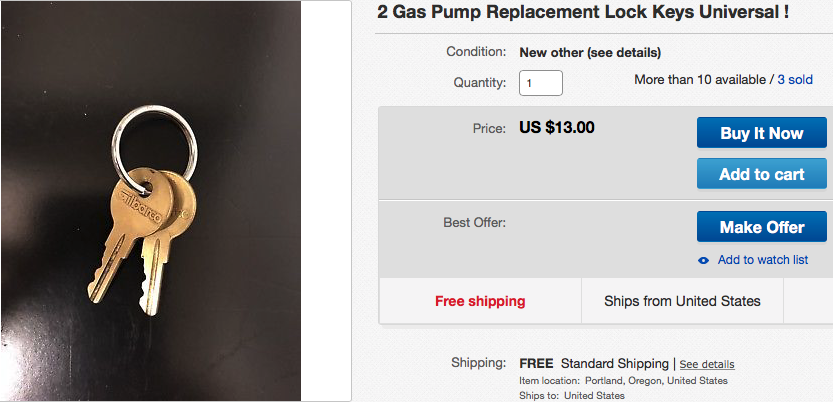
\includegraphics[width=\linewidth]{fig/universalkey.png}\\
    \caption{Criminals can buy keys for dispensers online.}
    \label{fig:universalkey}
\end{figure}

\paragraph{Fuel dispenser locks} Because fuel dispensers have not, historically, contained anything of value, their physical security was limited to using special ``security'' screws to prevent casual vandalism. The addition of a PoS terminal created an unforeseen incentive to break into a fuel dispenser, leaving dispenser makers to play catch up. In early versions of the Wayne Ovation fuel dispenser, for example, the perpetrator needs only to remove two screws on the front door to gain access to the inside, while Wayne Vista dispensers can be forced open with a screwdriver~\cite{ny-fuel-paymentdoor-access}. Only slightly harder to open are dispensers such as the Gilbarco Advantage, Gilbarco Encore 300 and Gilbarco 500s that use a single master key easily purchased on eBay (Figure~\ref{fig:universalkey}). 

While newer dispensers, such as the Wayne Helix and Gilbarco Encore 700~S, offer better physical security, a new fuel dispenser costs \$XXX--XXX, making dispenser upgrades are a costly undertaking for the approximately 150,000 fuel
stations in the US~\cite{npn-station-count}, the vast majority of which are independently owned and operated.

% (In Section~\ref{}, we show that 80\% of fuel stations in the US are still using vulnerable fuel dispenser models.)

\begin{figure}
    \centering
    \begin{minipage}{\linewidth}
        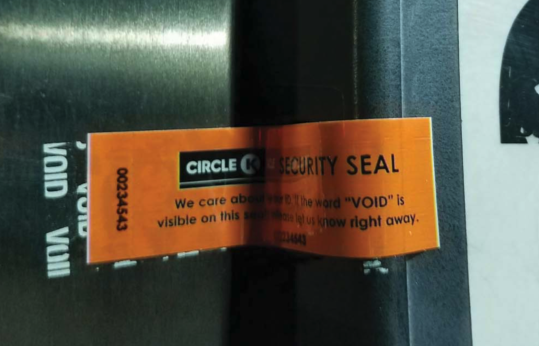
\includegraphics[height=0.33\linewidth,width=0.495\linewidth]{fig/branded_seal_untampered.png}\hfill
        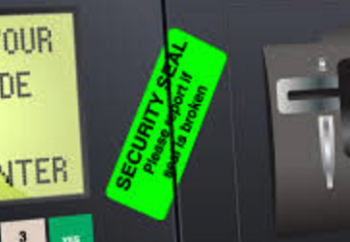
\includegraphics[height=0.33\linewidth,width=0.495\linewidth]{fig/unbranded_untampered.png}
    \end{minipage}
    \vskip1pt
    \begin{minipage}{\linewidth}
        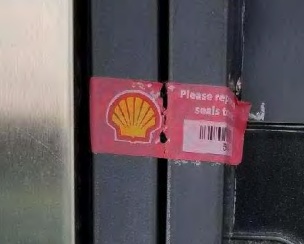
\includegraphics[height=0.33\linewidth,width=0.495\linewidth]{fig/branded_tampered_seal.png}\hfill
        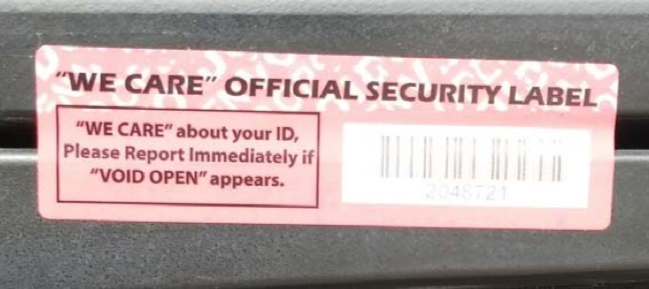
\includegraphics[height=0.33\linewidth,width=0.495\linewidth]{fig/unbranded_tampered_seal.png}
    \end{minipage}
    \vskip1pt
    \begin{minipage}{\linewidth}
        \fbox{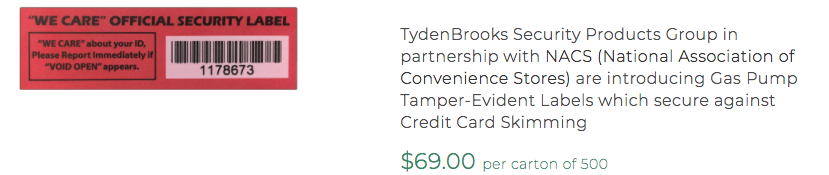
\includegraphics[width=0.97\linewidth]{fig/tamperseal.png}}
    \end{minipage}
    \caption{Tamper-evident seals used on fuel dispensers: (a) branded station seal, (b) generic (unbranded) seal, (c) trace of removed seal, and (d) generic seals available online for purchase.}
    \label{fig:seals}
\end{figure}

\paragraph{Tamper-evident seals} Fuel stations, especially those in areas where skimmers are common, are also starting to use tamper-evidence seals on their dispensers. The tamper-evident seal is applied across removable panels of the pump, and, if removed, leaves a visible trace (Figure~\ref{fig:tamperseal}(a-c)). As a customer-facing security measure, tamper-evident seals offer little protection: skimmer installers have been reported to repair broken seals using adhesive tape~\cite{} or replace the seals with generic versions (Figure~\ref{fig:seals}(d)). \noteby{KL}{Confirm claim about repair, ideally with reference. Any reports of replacement with generic seals in the wild?} On the other hand, regular inspection of seal integrity and authenticity by a station attendant may provide timely indication of tampering. It is important, however, that inspecting attendant should receive proper training on how to find skimmers. If, upon inspection, the attendant does not find a well-camouflaged skimmer (Figure~\ref{fig:wrapped-skimmer}), concludes that the damaged seal was a result of vandalism, and re-seals the dispenser with a new seal, all benefits of tamper-evident seals will be lost. This scenario is not so far fetched: in our own experience, well-trained field agents have missed skimmers that were then found on second inspection (Section~\ref{}). \noteby{KL}{Add reference to section discussing value of \bluetana\ at finding overlooked skimmers.}

\paragraph{Internal data encryption and chip cards} An alternative to preventing access to PoS terminal internals is to secure magnetic stripe data before it leaves the card reader itself, which would defeat the current generation of internal skimmers that attach to the cable between card reader and PoS terminal. This requires a costly upgrade to the PoS terminal, so such card readers are still only found in a small fraction of all vulnerable dispensers.

One of the forces driving PoS terminal upgrades is support for EMV cards, colloquially called \emph{chip cards}. While use of the chip itself does not protect against credit card information theft,\footnote{EMV cards have the same data stored on the chip as on the magnetic stripe, and this data can be extracted from the chip using so-called credit card \emph{shimmers}~\cite{krebshimmer}. While this data cannot be used to clone a correctly implemented EMV card, it is possible to create a card with the same data on the magnetic stripe as the original. Such a card can then still be used at merchants that use magnetic stripe (and not EMV chip) readers. EMV cards are intended to provide assurance to the merchant that the card is genuine; they do not protect the consumer from credit card data theft.} support for EMV requires a new PoS terminal, and such terminals typically offer better security features, including data encryption between reader and terminal. We are not aware of any reports of skimmers in EMV-capable fuel dispensers.

